\chapter{Stochastic Integration}\label{chap11}

LET\pageoriginale $\{X_{t}:t\geq 0\}$ BE A one-dimensional Brownian
motion. We want first to define integrals of the type
$\int\limits^{\infty}_{0}f(s)dX(s)$ for real functions $f\in
L^{1}[0,\infty)$. If $X(s,w)$ is of bounded variation almost
  everywhere then we can give a meaning to
  $\int\limits^{\infty}_{0}f(s)dX(s,w)=g(w)$. However, since $X(s,w)$
  is not bounded variation almost everywhere, $g(w)$ is not defined in
  the usual sense.

In order to define $g(w)=\int\limits^{\infty}_{0}f(s)dX(s,w)$ proceed
as follows.

Let $f$ be a step function of the following type:
$$
f=\sum\limits^{n}_{i=1}a_{i}X_{[t_{i},t_{i+1})}, 0\leq
  t_{1}<t_{2}<\ldots<t_{n+1}. 
$$

We naturally define
\begin{align*}
g(w)=\int\limits^{\infty}_{0}f(s)dX(s,w) &=
\sum\limits^{n}_{i=1}a_{i}(X_{t_{i+1}}(w)-X_{t_{i}}(w))\\
&= \sum\limits^{n}_{i=1}a_{i}(w(t_{i+1})-w(t_{i})).
\end{align*}
$g$ satisfies the following properties:
\begin{itemize}
\item[(i)] $g$ is a random variable;

\item[(ii)] $E(g)=0$; $E(g^{2})=\sum a^{2}_{i}(t_{i+1}-t_{i})=||f||_{2}$.
\end{itemize}

This follows from the facts that (a) $X_{t_{i+1}}-X_{t_{i}}$ is a
normal random variable with mean $0$ and variance $(t_{i+1}-t_{i})$
and (b) $X_{t_{i+1}}-X_{t_{i}}$ are independent increments, i.e.\@ we
have
$$
E\left(\int\limits^{\infty}_{0}fdX\right)=0,\ E\left(|\int\limits^{\infty}_{0}fdX |^{2}\right)=||f||^{2}_{2}.
$$\pageoriginale

\setcounter{exercise}{0}
\begin{exercise}\label{chap11-exer1}
If
\begin{align*}
& f=\sum\limits^{n}_{i=1}a_{i}X_{[t_{i},t_{i+1})}, 0\leq
    t_{1}<\ldots<t_{n+1},\\
& g=\sum\limits^{m}_{i=1}b_{i}X_{[s_{i},s_{i+1})}, 0\leq s_{1}<\ldots<s_{m+1},
\end{align*}

Show that
$$
\int\limits^{\infty}_{0}(f+g)dX(s,w)=\int\limits^{\infty}_{0}fdX(s,w)+\int\limits^{\infty}_{0}gdX(s,w)
$$
and 
$$
\int\limits^{\infty}_{0}(\alpha
f)dX(s,w)=\alpha\int\limits^{\infty}_{0}fdX(s,w),\ \forall \alpha\in
\mathbb{R}. 
$$
\end{exercise}

\begin{remark*}
The mapping $f\to \int\limits^{\infty}_{0}fdX$ is therefore a linear
$L^{2}_{\mathbb{R}}$-isometry of the space $S$ of all simple functions
of the type
$$
\sum^{n}_{i=1}a_{i}X_{[t_{i},t_{i+1})},(0\leq t_{1}<\ldots<t_{n+1})
$$
into $L^{2}(\Omega,\mathscr{B},P)$.
\end{remark*}

\begin{exercise}\label{chap11-exer2}
Show that $S$ is a dense subspace of $L^{2}[0,\infty)$. 

\noindent
Hint:~ $C_{c}[0,\infty)$, i.e.\@ the set of all continuous functions
  with compact support, is dense in $L^{2}[0,\infty)$. Show that $S$
    contains the closure of $C_{c}[0,\infty)$.
\end{exercise}

\begin{remark*}
The mapping $f\to \int\limits^{\infty}_{0}fdX$ can now be uniquely
extended as an isometry of $L^{2}[0,\infty)$ into
  $L^{2}(\Omega,\mathscr{B},P)$. 

Next\pageoriginale we define integrals fo the type
$$
g(w)=\int\limits^{t}_{0}X(s,w)dX(s,w)
$$

Put $t=1$ (the general case can be dealt with similarly). It seems
natural to define
\begin{equation*}
\int\limits^{1}_{0}X(s,w)dX(s)=\Lt\limits_{\sup |t_{j}-t_{j-1}|\to
  0}\sum\limits^{n}_{j=1}X(\xi j)(X(t_{j})-X(t_{j-1}))\tag{*}
\end{equation*}
where $0=t_{0}<t_{1}<\ldots <t_{n}=1$ is a partion of $[0,1]$ with
$t_{j-1}\leq \xi_{j}\leq t_{j}$. In general the limit on the right
hand side may not exist. Even if it exists it may happen that
depending on the choice of $\xi_{j}$, we may obtain different
limits. To consider an example we choose $\xi_{j}=t_{j}$ and then
$\xi_{j}=t_{j-1}$ and compute the right hand side of $(*)$. If
$\xi_{j}=t_{j-1}$, 
\begin{align*}
&\sum\limits^{n}_{j=1}X_{\xi_{j}}(X_{t_{j}}-X_{t_{j-1}})=\sum\limits^{n}_{j=1}X_{t_{j-1}}-(X_{t_{j}}-X_{t_{j-1}})\\
&\qq
  =\frac{1}{2}\sum\limits^{n}_{j=1}(X_{t_{j}})-(X_{t_{j-1}})-\frac{1}{2}\sum\limits^{n}_{j=1}(X_{t_{j}}-X_{t_{j-1}})\\
& \frac{1}{2}[X^{2}(1)-X^{2}(0)]-\frac{1}{2}\text{~ as~ } n\to \infty,
  \text{~ and~ } \sup |t_{j}-t_{j-1}|\to 0,
\end{align*}
arguing as in the proof of the result that Brownian motion is not of
bounded variation. If $\xi_{j}=t_{j}$,
$$
\Lt\limits_{\substack{n\to \infty\\ \Sup |t_{j}-t_{j-1}|\to 0}}\sum^{n}_{j=1}X_{t_{j}}(X_{t_{j}}-X_{t_{j-1}})=1/2X(1)-1/2X(0)+1/2.
$$

Thus\pageoriginale we get different answers depending on the choice of
$\xi_{j}$ and hence one has to be very careful in defining the
integral. It turns out that the choice of $\xi_{j}=t_{j-1}$ is more
appropriate in the definition of the integral and gives better results.
\end{remark*}

\begin{remark*}
The limit in $(*)$ should be understood in the sense of convergence
probability. 
\end{remark*}

\begin{exercise}\label{chap11-exer3}
Let $0\leq a<b$. Show that the ``left integral'' $(\xi_{j}=t_{j-1})$
is given by
$$
L\int\limits^{b}_{a}X(s)dX(s)=\frac{X^{2}(b)-X^{2}(a)-(b-a)}{2}
$$
and the ``right integral'' $(\xi_{j}=t_{j})$ is given by
$$
R\int\limits^{b}_{s}X(s)dX(s)=\frac{X^{2}(b)-X^{2}(a)+(b-a)}{2}.
$$

We now take up the general theory of stochastic integration. To
motivate the definitions which follow let us consider a
$d$-dimensional Brownian motion $\{\beta(t):t\geq 0\}$. We have
$$
E[\beta(t+s)-\beta(t)\in
  A|\mathscr{F}_{t}]=\int\limits_{A}1/\surd(2\pi s)e^{-|y|^{2}/2s}dy.
$$

Thus
$$
E(f(\beta(t+s)-\beta(t))|\mathscr{F}_{t}]=\int f(y)1/\surd(2\pi
s)e^{-|y|^{2/2s}}dy. 
$$

In particular, if $f(x)=e^{ix.u}$,
\begin{align*}
E[e^{iu}(\beta(t+s)-\beta(t))|\mathscr{F}_{t}] &= \int e^{iu.y}1/\surd
(2\pi s)e^{-|y|^{2}/2s}dy\\
&= e^{\frac{-s|u|^{2}}{2}}.
\end{align*}

Thus\pageoriginale
$$
E[e^{iu.\beta(t+s)}|\mathscr{F}_{t}]=e^{iu.\beta(t)}e^{-s|u|^{2}/2},
$$
or,
$$
E[e^{iu.\beta(t+s)+(t+s)|u|^{2}/2}|\mathscr{F}_{t}]=e^{iu.\beta(t)+t|u|^{2}/2}.
$$

Replacing $iu$ by $\theta$ we get
$$
E[e^{\theta.\beta(s)-|s\theta|^{2}/2}\mid\mathscr{F}_{t}]=e^{\theta.\beta(t)-t|\theta|^{2/2}},
\ s>t, \forall \theta. 
$$

It is clear that $e^{\theta.\beta(t)-t|\theta|^{2}/2}$ is
$\mathscr{F}_{t}$-measurable and a simple calculation gives
$$
E(e^{\theta.\beta(t)-|\theta|^{2}t/2|})<\infty \ \forall \theta.
$$
\end{exercise}

We thus have

\begin{theorem*}
If $\{\beta(t):t\geq 0\}$ is a $d$-dimensional Brownian motion then
$\exp [\theta.\beta(t)-|\theta|^{2}t/2]$ is a Martingale relative to
$\mathscr{F}_{t}$, the $\sigma$-algebra generated by $(\beta(s):s\leq t)$.
\end{theorem*}

\begin{defi*}
Let $(\Omega,\mathscr{B},P)$ be a probability space
$(\mathscr{F}_{t})_{t\geq 0}$ and increasing family of
sub-$\sigma$-algebras of $\mathscr{F}$ with
$\mathscr{F}=\sigma(\bigcup\limits_{t\geq 0}\mathscr{F}_{t})$. 

Let
\begin{itemize}
\item[(i)] $a:[0,\infty)\times \Omega\to [0,\infty)$ be bounded and
    progressively measurable;

\item[(ii)] $b:[0,\infty)\times \Omega\to \mathbb{R}$ be bounded and
  progressively measurable;

\item[(iii)] $X:[0,\infty)\times \Omega\to \mathbb{R}$ be
  progressively measurable, right continuous on $[0,\infty)$,
    $\forall\ w\in \Omega$, and continous on $[0,\infty)$ almost
      everywhere on $\Omega$;

\item[(iv)] $Z_{t}(w)=e^{\theta
  X(t,w)-\theta\int\limits^{t}_{0}b(s,w)ds-\frac{\theta^{2}}{2}\int\limits^{t}_{0}a(s,w)ds}$\pageoriginale

be a Martingale relative to $(\mathscr{F}_{t})_{t\geq 0}$.
\end{itemize}
\end{defi*}

Then $X(t,w)$ is called an Ito process corresponding to the
parameters $b$ and $a$ and we write $X_{t}\in I[b,a]$.

\medskip
\noindent
{\bf N.B.}~ The progressive measurability of $X\Rightarrow X_{t}$ is
$\mathscr{F}_{t}$-measurable.

\begin{example*}
If $\{\beta(t):t\geq 0\}$ is a Brownian motion, then
$X(t,w)=\beta_{t}(w)$ is an Ito process corresponding to parameters
$0$ and $1$. (i) and (ii) are obvious. (iii) follows by right
continuity of $\beta_{t}$ and measurability of $\beta_{t}$ relative to
$\mathscr{F}_{t}$ and (iv) is proved in the previous theorem.
\end{example*}

\begin{exercise}\label{chap11-exer4}
Show that $Z_{t}(w)$ defined in (iv) is $\mathscr{F}_{t}$-measurable
and progressively measurable.
\end{exercise}

\noindent
[Hint: 
\begin{itemize}
\item[(i)] $Z_{t}$ is right continuous.

\item[(ii)] Use Fubini's theorem to prove measurability].
\end{itemize}

\begin{remark*}
If we put $Y(t,w)=X(t,w)-\int\limits^{t}_{0}b(s,w)ds$ then $Y(t,w)$ is
progressively measurable and $Y(t,w)$ is an Ito process corresponding
to the parameters $0$, $a$. Thus we need only consider integrals of
the type $\int\limits^{t}_{0}f(s,w)dY(s,w)$ and {\em define}
$$
\int\limits^{t}_{0}f(s,w)dX(s,w)=\int\limits^{t}_{0}f(s,w)dY(s,w)+\int\limits^{t}_{0}f(s,w)b(s,w)ds.
$$
(Note that {\em formally} we have $dY=dX-dbt$).
\end{remark*}

\begin{lemma*}
If\pageoriginale $Y(t,w)\in I[0,a]$, then
$$
Y(t,w)\quad\text{and}\quad Y^{2}(t,w)-\int\limits^{t}_{0}a(s,w)ds
$$
are Martingales relative to $(\mathscr{F}_{t})$.
\end{lemma*}

\begin{proof}
To motivate the arguments which follow, we first give a formal proof. Let
$$
Y_{\theta}(t)=e^{\theta Y(t,w)-\frac{\theta^{2}}{2}\int\limits^{t}_{0}a(s,w)ds}.
$$

Then $Y_{\theta}(t)$ is a martingale, $\forall \theta$. Therefore
$\dfrac{Y_{\theta}-1}{\theta}$ is a Martingale, $\forall
\theta$. Hence (formally),
$$
\lim\limits_{\theta\to
  0}\dfrac{Y_{\theta}-1}{\theta}=Y'_{\theta}|_{\theta=0}
$$
is a Martingale.

\setcounter{step}{0}
\begin{step}%1
$Y(t,\cdot)\in L^{k}(\Omega,\mathscr{F},P)$, $k=0,1,2,\ldots$ and
  $\forall t$. In fact, for every real $\theta$, $Y_{\theta}(t)$ is a
  Martingale and hence $E(Y_{\theta})<\infty$. Since $a$ is bounded
  this means that
$$
E(e^{\theta Y(t,\cdot)})<\infty,\ \forall \theta.
$$

Taking $\theta=1$ and $-1$ we conclude that $E(e^{|Y|})<\infty$ and
hence $E(|Y|^{k})<\infty$, $\forall k=0,1,2,\ldots$. Since $Y$ is an
Ito process we also get
$$
\sup\limits_{|\theta|\leq
  \alpha}E\left(\left[e^{Y(t,\cdot)-\frac{\theta^{2}}{2}\int\limits^{t}_{0}ads}\right]^{k}\right)<\infty
$$
$\forall k$ and for every $\alpha>0$.
\end{step}

\begin{step}%2
Let\pageoriginale
$X_{\theta}(t)=[Y(t,\cdot)-\theta\int\limits^{t}_{0}ads]Y(t)=\dfrac{d}{d\theta}Y_{\theta}(t,\cdot)$. 

Define
$$
\phi_{A}(\theta)=\int\limits_{A}(X_{\theta}(t,\cdot)-X_{\theta}(s,\cdot))dP(w)
$$
where $t>s$, $A\in\mathscr{F}_{s}$. Then
$$
\int\limits^{\theta_{2}}_{\theta_{1}}\phi_{A}(\theta)d\theta=\int\limits^{\theta_{2}}_{\theta_{1}}\int\limits_{A}[X_{\theta}(t,\cdot)-X_{\theta}(S,\cdot)]dP(w)d\theta. 
$$

Since $a$ is bounded, $\sup\limits_{|\theta|\leq
  \alpha}E([Y_{\theta}(t,\cdot)]^{k})<\infty$, and
$E(|Y|^{k})<\infty$, $\forall k$; we can use Fubini's theorem to get
\begin{gather*}
\int\limits^{\theta_{2}}_{\theta_{1}}\phi_{A}(\theta)d\theta=\int\limits_{A}\int\limits^{\theta_{2}}_{\theta_{1}}[X_{\theta}(t,\cdot)-X_{\theta}(s,\cdot)]d\theta\ dP(w). 
\end{gather*}
or
$$
\int\limits^{\theta_{2}}_{\theta_{1}}\phi_{A}(\theta)d\theta=\int\limits_{A}Y_{\theta_{2}}(t,\cdot)-Y_{\theta_{1}}(t,\cdot)dP(w)-\int\limits_{A}Y_{\theta_{1}}(s,\cdot)-Y_{\theta_{1}}(s,\cdot)dP(w). 
$$

Let $A\in\mathscr{F}_{s}$ and $t>s$; then, since $Y$ is a Martingale,
$$
\int\limits^{\theta_{2}}_{\theta_{1}}\phi_{A}(\theta)d\theta=0.
$$

This is true $\forall \theta_{1}<\theta_{2}$ and since
$\phi_{A}(\theta)$ is a continuous function of $\theta$, we conclude
that
$$
\phi_{A}(\theta)=0,\ \forall \theta.
$$

In particular, $\phi_{A}(\theta)=0$ which means that
$$
\int\limits_{A}Y(t,\cdot)dP(w)=\int\limits_{A}Y(s,\cdot)dP(w),\ \forall
A\in \mathscr{F}_{s},\ t>s,
$$
i.e.,\pageoriginale $Y(t)$ is a Martingale relative to $(\Omega,\mathscr{F}_{t},P)$.
\end{step}

To prove the second part we put
$$
Z_{\theta}(t,\cdot)=\frac{d^{2}}{d\theta^{2}}Y_{\theta}(t)
$$
and 
$$
\psi_{A}(\theta)=\int\limits_{A}\{Z_{\theta}(t,\cdot)-Z_{\theta}(s,\cdot)\}dP(w). 
$$

Then, by Fubini,
$$
\int\limits^{\theta_{2}}_{\theta_{1}}\psi_{A}(\theta)d\theta=\int\limits_{A}\int\limits^{\theta_{2}}_{\theta_{1}}Z_{\theta}(t,\cdot)-Z_{\theta}(s,\cdot)d\theta\ dP(w). 
$$
or,
\begin{align*}
\int\limits^{\theta_{2}}_{\theta_{1}}\psi_{A}(\theta)d\theta
&=\phi_{A}(\theta_{2})-\phi_{A}(\theta_{1})\\
&= 0\text{~ if~ } A\in \mathscr{F}_{s},\ t>s.
\end{align*}

Therefore
$$
\psi_{A}(\theta)=0,\ \forall \theta.
$$

In particular, $\psi_{A}(\theta)=0$ implies that
$$
Y^{2}(t,w)-\int\limits^{t}_{0}a(s,w)ds
$$
is an $(\Omega,\mathscr{F}_{t},P)$ Martingale. This completes the
proof of lemma \ref{chap8-lem1}.
\end{proof}

\begin{defi*}
A function $\theta:[0,\infty)\times \Omega\to \mathbb{R}$ is called
  simple if there exist reals $s_{0}$, $s_{1},\ldots,s_{n},\ldots$
$$
0\leq s_{0}<s_{1}<\ldots<s_{n}\ldots<\infty,
$$
$s_{n}$ increasing to $+\infty$ and
$$
\theta(s,w)=\theta_{j}(w)
$$\pageoriginale
if $s\in [s_{j},s_{j+1})$, where $\theta_{j}(w)$ is
  $\mathscr{F}_{s_{j}}$-measurable and bounded.
\end{defi*}

\begin{defi*}
Let $\theta:[0,\infty)\times \Omega\to \mathbb{R}$ be a simple
  function and $Y(t,w)\in I[0,a]$. We define the stochastic integral
  of $\theta$ with respect to $Y$, denoted
$$
\int\limits^{t}_{0}\theta(s,w)dY(s,w)),
$$
by
\begin{align*}
\xi(t,w) &= \int\limits^{t}_{0}\theta(s,w)dY(s,w)\\
&=
\sum\limits^{k}_{j=1}\theta_{j-1}(w)[Y(s_{j},w)-Y(s_{j-1},w)]+\theta_{k}(w)[Y(t,w)-Y(s_{k},w)]. 
\end{align*}
\begin{figure}[H]
\centering
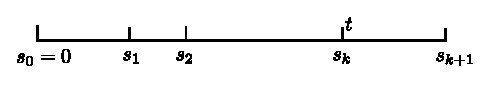
\includegraphics{figure/fig9.eps}
\end{figure}
\end{defi*}

\setcounter{lemma}{1}
\begin{lemma}\label{chap11-lem2}
Let $\sigma:[0,\infty)\times\Omega\to \mathbb{R}$ be a simple function
  and $Y(t,w)\in I[0,a]$. Then
$$
\xi(t,w)=\int\limits^{t}_{0}\sigma(s,w)dY(s,w)\in I[0,a\sigma^{2}].
$$
\end{lemma}

\begin{proof}
\begin{enumerate}
\renewcommand{\theenumi}{\roman{enumi}}
\renewcommand{\labelenumi}{(\theenumi)}
\item By definition, $\sigma$ is right continuous and $\sigma(t,w)$ is
  $\mathscr{F}_{t}$-measurable; hence it is progressively
  measurable. Since $a$ is progressively measurable and bounded
$$
a\sigma^{2}:[0,\infty)\times \Omega\to [0,\infty)
$$
is progressively measurable and bounded.

\item From\pageoriginale the definition of $\xi$ it is clear that
  $\xi(t,\cdot)$ is right continuous, continous almost everywhere and
  $\mathscr{F}_{t}$-measurable therefore $\xi$ is progressively
  measurable.

\item
  $Z_{t}(w)=e^{[\theta\xi(t,w)-\frac{\theta^{2}}{2}\int\limits^{t}_{0}a\sigma^{2}ds]}$ 

is clearly $\mathscr{F}_{t}$-measurable $\forall \theta$. We show that
$$
E(Z_{t})<\infty,\ \forall t\text{~ and~ }
E(Z_{t_{2}}|\mathscr{F}_{t_{1}})=Z_{t_{1}}\text{~ if~ }t_{1}<t_{2}.
$$
\end{enumerate}

We can assume without loss of generality that $\theta=1$ (if
$\theta\neq 1$ we replace $\sigma$ by $\theta\sigma$). Therefore
$$
Z_{t}(w)=e^{[\xi(t,w)-\int\limits^{t}_{0}a\sigma^{2}ds]}.
$$
Since $a$ and $\sigma$ are bounded uniformly on $[0,t]$, it is enough
to show that $E(e^{\xi(t,w)})<\infty$. By definition,
$$
\xi(t,w)=\sum\limits^{k}_{j=1}\theta_{j-1}(w)[Y(s_{j},w)-Y(s_{j-1},w)]+\theta_{k}(w)(Y(t,w)-Y(s_{k},w)).
$$
The result $E(e^{\xi(t,w)})<\infty$ will follow from the generalised
Holder's inequality provided we show that
$$
E(e^{\theta(w)[Y(t,w)-Y(s,w)]})<\infty
$$
for every bounded function $\theta$ which is
$\mathscr{F}_{s}$-measurable. Now
$$
E(e^{\theta[Y(t,\cdot)-Y(s,\cdot)]}|\mathscr{F}_{s})=
$$ 
constant for every constant $\theta$, since $Y\in I[0,a]$. Therefore
$$
E(e^{\theta(w)[Y(t,\cdot)-Y(s,\cdot)]}|\mathscr{F}_{s})=\text{~constant}
$$
for\pageoriginale every $\theta$ which is bounded and
$\mathscr{F}_{s}$-measurable. Thus
$$
E(e^{\theta(w)[Y(t,\cdot)-Y(s,\cdot)]})<\infty.
$$

This proves that $E(Z_{t}(w))\in \infty$. 

Finally we show that
$$
E(Z_{t_{2}}|\mathscr{F}_{t_{1}})=Z_{t_{1}}(w),\q\text{if}\q
t_{1}<t_{2}.
$$

Consider first the case when $t_{1}$ and $t_{2}$ are in the same
interval 
$$
[s_{k},s_{k+1}).
$$ 
Then
\begin{align*}
& \xi(t_{2},w)=\xi(t_{1},w)+\sigma_{k}(w)[Y(t_{2},w)-Y(t_{1},w)]\q\text{(see
  definition),}\\
& \int\limits^{t_{2}}_{0}a\sigma^{2}(s,w)ds=\int\limits^{t_{1}}_{0}a\sigma^{2}(s,w)ds+\int\limits^{t_{2}}_{t_{1}}a\sigma^{2}(s,w)ds.
\end{align*}

Therefore
{\fontsize{10pt}{12pt}\selectfont
$$
E(Z_{t_{2}}(w)|\mathscr{F}_{t_{1}})=Z_{t_{1}}(w)E(\exp[\theta\sigma_{k}(w)[Y(t_{2},w)-Y(t_{1},w)]-\frac{\theta^{2}}{2}\int\limits^{t_{2}}_{t_{1}}a\sigma^{2}ds)|\mathscr{F}_{t_{1}}) 
$$}\relax
as $Y\in I[0,a]$.
\begin{equation*}
E(\exp[\theta(Y(t_{2},w)-T(t_{1},w))-\frac{\theta^{2}}{2}\int\limits^{t_{2}}_{t_{1}}a(s,w)ds]|\mathscr{F}_{t_{1}})=1\tag{*}
\end{equation*}
and since $\sigma_{k}(w)$ is $\mathscr{F}_{t_{1}}$-measurable $(*)$
remains valid if $\theta$ is replaced by $\theta\sigma_{k}$. Thus
$$
E(Z_{t_{2}}|\mathscr{F}_{t_{1}})=Z_{t_{1}}(w).
$$

The general case follows if we use the identity
$$
E(E(X|\mathscr{C}_{1})|\mathscr{C}_{2})=E(X|\mathscr{C}_{2})\quad\text{for}\quad
\mathscr{C}_{2}\subset \mathscr{C}_{1}.
$$

Thus $Z_{t}$ is a Martingale and $\xi(t,w)\in I[0,a\sigma^{2}]$.
\end{proof}

\begin{coro*}
\begin{itemize}
\item[(i)] $\xi(t,w)$\pageoriginale is a martingale; $E(\xi(t,w))=0$;

\item[(ii)] $\xi^{2}(t,w)-\int\limits^{t}_{0}a\sigma^{2}ds$

is a Martingale with
$$
E(\xi^{2}(t,w))=E(\int\limits^{t}_{0}a\sigma^{2}(s,w)ds.
$$
\end{itemize}
\end{coro*}

\begin{proof}
Follows from Lemma \ref{chap8-lem1}.
\end{proof}

\begin{lemma}\label{chap11-lem3}
Let $\sigma(s,w)$ be progressively measurable such that for each $t$,
$$
E(\int\limits^{t}_{0}\sigma^{2}(s,w)ds)<\infty.
$$

Then there exists a sequence $\sigma_{n}(s,w)$ of simple functions
such that
$$
\lim\limits_{n\to \infty}E\left(\int\limits^{t}_{0}|\sigma_{n}(s,w)-\sigma(s,w)|^{2}ds\right)=0.
$$
\end{lemma}

\begin{proof}
We may assume that $\sigma$ is bounded, for if $\sigma_{N}=\sigma$ for
$|\sigma|\leq N$ and $0$ if $|\sigma|>N$, then $\sigma_{n}\to \sigma$,
$\forall (s,w)\in [0,t]\times\Omega$. $\sigma_{N}$ is progressively
measurable and $|\sigma_{n}-\sigma|^{2}\leq 4|\sigma|^{2}$. By
hypothesis $\sigma\in L([0,t]:\Omega)$.

Therefore $E(\int\limits^{t}_{0}|\sigma_{n}-\sigma|ds)\to 0$, by
dominated convergence. Further, we can also assume that $\sigma$ is
continuous. For, if $\sigma$ is bounded, define
$$
\sigma_{h}(t,w)=1/h\int\limits^{t}_{(t-h)v0}\sigma(s,w)ds.
$$
$\sigma_{n}$ is continuous in $t$ and $\mathscr{F}_{t}$-measurable and
hence progressively measurable. Also by Lebesgue's theorem
$$
\sigma_{h}(t,w)\to \sigma(t,w),\quad\text{as}\quad h\to 0,\forall t,w.
$$

Since\pageoriginale $\sigma$ is bounded by $C$, $\sigma_{h}$ is also
bounded by $C$. Thus
$$
E(\int\limits^{t}_{0}|\sigma_{h}(s,w)-\sigma(s,w)|^{2}ds)\to 0.
$$
(by dominated convergence). If $\sigma$ is continuous, bounded and
progressively measurable, then
$$
\sigma_{n}(s,w)=\sigma\left(\frac{[ns]}{n},w\right)
$$
is progressively measurable, bounded and simple. But
$$
\Lt\limits_{n\to \infty}\sigma_{n}(s,w)=\sigma(s,w).
$$

Thus by dominated convergence
$$
E\left(\int\limits^{t}_{0}|\sigma_{n}-\sigma|^{2}ds\right)\to
0\quad\text{as}\quad n\to \infty.
$$
\end{proof}


\begin{theorem*}
Let $\sigma(s,w)$ be progressively measurable, such that
$$
E(\int\limits^{t}_{0}\sigma^{2}(s,w)ds)<\infty
$$ 
for each $t>0$. Let
$(\sigma_{n})$ be simple approximations to $\sigma$ as in Lemma
\ref{chap11-lem3}. Put
$$
\xi_{n}(t,w)=\int\limits^{t}_{0}\sigma_{n}(s,w)dY(s,w)
$$
where $Y\in I[0,a]$. Then
\begin{itemize}
\item[\rm(i)] $\Lt\limits_{n\to \infty}\xi_{n}(t,w)$ exists uniformly
  in probability, i.e.\@ there exists an almost surely continuous
  $\xi(t,w)$ such that
$$
\Lt\limits_{n\to \infty}P\left(\sup\limits_{0\leq t\leq
  T}|\xi_{n}(t,w)-\xi(t,w)|\geq \epsilon\right)=0
$$
for each $\epsilon>0$ and for each $T$. Moreover, $\xi$ is independent
of the sequence $(\sigma_{0})$.

\item[\rm(ii)] The\pageoriginale map $\sigma\to \xi$ is linear.


\item[\rm(iii)] $\xi(t,w)$ and
  $\xi^{2}(t,w)-\int\limits^{t}_{0}a\sigma^{2}ds$ are Martingales.

\item[\rm(iv)] If $\sigma$ is bounded, $\xi\in I[0,a\sigma^{2}]$.
\end{itemize}
\end{theorem*}

\begin{proof}
\begin{enumerate}
\renewcommand{\theenumi}{\roman{enumi}}
\renewcommand{\labelenumi}{(\theenumi)}
\item It is easily seen that for simple functions the stochastic
  integral is linear. Therefore
$$
(\xi_{n}-\xi_{m})(t,w)=\int\limits^{t}_{0}(\sigma_{n}-\sigma_{m})(s,w)dY(s,w).
$$

Since $\xi_{n}-\xi_{m}$ is an almost surely continuous martingale
$$
P\left(\sup\limits_{0\leq t\leq T}|\xi_{n}(t,w)-\xi_{m}(t,w)|\geq
\epsilon\right)\leq \frac{1}{\epsilon^{2}}E[(\xi_{n}-\xi_{m})^{2}(T,w)].
$$

This is a consequence of Kolmogorov inequality (See Appendix). Since
$$
(\xi_{n}-\xi_{m})^{2}-\int\limits^{t}_{0}a(\sigma_{n}-\sigma_{m})^{2}ds
$$
is a Martingale, and $a$ is bounded,
\begin{align*}
E[(\xi_{n}-\xi_{m})^{2}(T,w)] &=
E\left(\int\limits^{T}_{0}(\sigma_{n}-\sigma_{m})^{2}a\ ds\right).\tag{*}\\
&\leq \text{const\,}\frac{1}{\epsilon^{2}}E\left(\int\limits^{T}_{0}(\sigma_{n}-\sigma_{m})^{2}ds\right).
\end{align*}

Therefore
$$
\Lt\limits_{n,m\to \infty}E[(\xi_{n}-\xi_{m})^{2}(T,w)]=0.
$$

Thus $(\xi_{n}-\xi_{m})$ is uniformly Cauchy in probability. Therefore
there exists a progressively measurable $\xi$ such that 
$$
\Lt\limits_{n\to\infty}P\left(\sup\limits_{0\leq t\leq
  T}|\xi_{n}(t,w)-\xi(t,w)|\geq \epsilon\right)=0,\ \forall
\epsilon>0,\ \forall T.
$$

It can be shown that $\xi$ is almost surely continuous.

If\pageoriginale $(\sigma_{n})$ and $(\sigma'_{n})$ are two sequences
of simple functions approximating $\sigma$, then $(*)$ shows that
$$
E[(\xi_{n}-\xi'_{n})^{2}(T,w)]\to 0.
$$

Thus
$$
\Lt\limits_{n}\xi_{n}=\Lt\limits_{n}\xi'_{n},
$$
i.e.\@ $\xi$ is independent of $(\sigma_{n})$.

\item is obvious.

\item (*) shows that $\xi_{n}\to \xi$ in $L$ and therefore
  $\xi_{n}(t,\cdot)\to \xi(t,\cdot)$ in $L^{1}$ for each fixed
  $t$. Since $\xi_{n}(t,w)$ is a martingale for each $n$, $\xi(t,w)$
  is a martingale.

\item $\xi^{2}_{n}(t,w)-\int\limits^{t}_{0}a\sigma^{2}_{n}$ is a
  martingale for each $n$.


Since $\xi_{n}(t,w)\to \xi(t,w)$ in $L^{2}$ for each fixed $t$ and
$$
\xi^{2}_{n}(t,w)\to \xi^{2}(t,w)\quad\text{in}\quad L^{1}\q\text{for
  each fixed~} t.
$$

For $\xi^{2}_{n}(t,w)-\xi^{2}(t,w)=(\xi_{n}-\xi)(\xi_{n}+\xi)$ and
using H\"older's inequality, we get the result.

Similarly, since
\begin{align*}
& \sigma_{n}\to \sigma\text{~ in~ } L^{2}([0,t]\times\Omega),\\
& \sigma^{2}_{n}\to \sigma^{2}\text{~ in~ }L^{1}([0,t]\times\Omega),
\end{align*}
and because $a$ is bounded $a\sigma^{2}_{n}\to a\sigma^{2}$ in
$L^{1}([0,t]\times\Omega)$. This shows that
$\xi^{2}_{n}(t,w)-\int\limits^{t}_{0}a\sigma^{2}_{n}ds$ converges to
$$
\xi^{2}(t,w)-\int\limits^{t}_{0}a\sigma^{2}ds
$$
for each $t$ in $L^{1}$. Therefore
$$
\xi^{2}(t,w)-\int\limits^{t}_{0}a\sigma^{2}ds
$$\pageoriginale
is a martingale.

\item Let $\sigma$ be bounded. To show that $\xi\in I[0,\sigma^{2}]$
  it is enough to show that
$$
e^{\theta\xi(t,w)-\frac{\theta^{2}}{2}\int\limits^{t}_{0}a\sigma^{2}ds}
$$
is a martingale for each $\theta$, the other conditions being
trivially satisfied. Let
$$
Z_{n}(t,w)=e^{\theta\xi_{n}(t,w)-\frac{\theta^{2}}{2}\int\limits^{t}_{0}a\sigma^{2}_{n}ds}
$$

We can assume that $|\sigma_{n}|\leq C$ if $|\sigma|\leq C$ (see the
proof of Lemma \ref{chap11-lem3}).
$$
Z_{n}=\exp\left[2\theta\xi_{n}(t,w)-\frac{(2\theta)^{2}}{2}\int\limits^{t}_{0}a\sigma^{2}_{n}ds+\theta^{2}\int\limits^{t}_{0}a\sigma^{2}_{n}ds\right].
$$

Thus
\begin{equation*}
E(Z_{n})\leq \text{const\,}E\left(e^{2\theta \xi_{n}(t,w)-\frac{(2\theta)^{2}}{2}\int\limits^{t}_{0}a\sigma^{2}_{n}ds}\right)=\text{const}\tag{**}
\end{equation*}
since $Z_{n}$ is a martingale for each $\theta$. A subsequence
$Z_{n_{i}}$ converges to
$$
e^{\theta\xi(t,w)-\frac{\theta^{2}}{2}\int\limits^{t}_{0}a\sigma^{2}ds}
$$
almost everywhere $(P)$. This together with (**) ensures uniform
integrability of $(Z_{n})$ and therefore
$$
e^{\theta\xi(t,w)-\frac{\theta^{2}}{2}\int\limits^{t}_{0}a\sigma^{2}ds}
$$
is a martingale. Thus $\xi$ is an Ito process, $\xi\in I[0,a\sigma^{2}]$.
\end{enumerate}
\end{proof}

\begin{defi*}
With the hypothesis as in the above theorem we define the stochastic
integral
$$
\xi(t,w)=\int\limits^{t}_{0}\sigma(s,w)dY(s,w).
$$\pageoriginale
\end{defi*}

\begin{exer*}
Show that $d(X+Y)=dX+dY$.
\end{exer*}

\begin{remark*}
If $\sigma$ is bounded, then $\xi$ satisfies the hypothesis of the
previous theorem and so one can define the integral of $\xi$ with
respect to $Y$. Further, since $\xi$ itself is It\^o, we can also
define stochastic integrals with respect to.
\end{remark*}

\begin{examples*}
\begin{enumerate}
\item
Let $\{\beta(t):t\geq 0\}$ be a Brownian motion; then $\beta(t,w)$ is
progressively measurable (being continuous and
$\mathscr{F}_{t}$-measurable). Also,
$$
\int\limits_{\Omega}\int\limits^{t}_{0}\beta^{2}(s)ds\ dP=\int\limits^{t}_{0}\int\limits_{\Omega}\beta^{2}(s)dP\ ds=\int\limits^{t}_{0}sds=\frac{t}{2}
$$

Hence
$$
\int\limits^{t}_{0}\beta(s,w)d\beta(s,w)
$$
is well defined.

\item Similarly $\int\limits^{t}_{0}\beta(s/2)d\beta(s)$ is well
  defined.

\item However
$$
\int\limits^{t}_{0}\beta(2s)d\beta(s)
$$
is not well defined, the reason being that $\beta(2s)$ is not
progressively measurable.
\end{enumerate}
\end{examples*}

\begin{exercise}\label{chap11-exer5}
Show\pageoriginale that $\beta(2s)$ is not progressively measurable. 

\noindent
(Hint:~ Try to show that $\beta(2s)$ is not
$\mathscr{F}_{s}$-measurable for every $s$. To show this prove that
$\mathscr{F}_{s}\neq \mathscr{F}_{2s}$).
\end{exercise}

\begin{exercise}\label{chap11-exer6}
Show that for a Brownian motion $\beta(t)$, the stochastic integral
$$
\int\limits^{1}_{0}\beta(s,\cdot)d\beta(s,\cdot)
$$
is the same as the left integral
$$
L\int\limits^{1}_{0}\beta(s,\cdot)d\beta(s,\cdot)
$$
defined earlier.
\end{exercise}
